\documentclass[../main.tex]{subfiles}

\begin{document}

\chapter{Формулювання та аналіз вимог до багтрекеру}

\section{Формулювання та аналіз вимог}

\subsection{Формулювання вимог}

Розглянувши існуючі на цей час програмні продукти для багтрекінгу, проаналізувавши їх, та виявивши як позитивні так і негативні їх сторони, можна сформулювати задачі розробки. В узагальненому вигляді такою задачею є створення програмного комплексу, що буде забезпечувати можливість легкого розгортання, підтримки та модифікації системи, а також надання публічного API для спілкування з клієнтами для будь-яких платформ.

При проектуванні програмного продукту необхідно забезпечити наступні можливості:
\begin{enumerate}
    \item Авторизація за допомогою внутрішнього аккаунта.
    \item Можливість управління проектами та їх учасниками.
    \item Можливість управління правами учасників проекту.
    \item Збереження даних щодо проблем/пропозицій.
    \item Можливість прикріплення додаткових артефактів до кожного звіту.
    \item Можливість написання клієнту під будь-яку платформу завдяки вікористанню розподіленої моделі взаємодії.
    \item Синхронізація між пристроями користувачів.
    \item Інтерфейсна частина клієнтського додатку повинна забезпечувати відображення списків проектів, проблем/пропозицій, інформації про проблему, додатків до проблеми.
\end{enumerate}

\subsection{Аналіз вимог}

\subsubsection{Авторизація за допомогою внутрішнього аккаунта}
% TODO % I think this leads to too large vertical spaces. Maybe it should be better to change such subsubsections (at least, so small subsubsections) to subparagraphs, with point at end. For example: \subparagraph{Авторизація за допомогою внутрішнього аккаунта.}
Для того, щоб багтрекінгова система працювала, кожний користувач повинен мати свій обліковий запис в базі даних. Серед варіантів реалізації авторизації є два основних підходи: використання власної бази облікових записів або використання стороннього сервісу облікових записів. Реалізація підходу з використанням стороннього сервісу авторизації має декілька проблем:
\begin{enumerate}
    \item Можливість зміни механізму авторизації третьою стороною (що автоматично унеможливлює авторизацію).
    \item Відсутність можливості контролю методу зберігання облікових записів та даних користувачів.
\end{enumerate}

Зважаючи на перелічені недоліки підходу зі стороннім сервісом авторизації було вирішено написати власну систему авторизації.

\subsubsection{Можливість управління проектами та їх учасниками}
Для функціонування багтрекінгової системи в умовах надання публічного API необхідно мати можливість логічного розподілення звітів серед існуючих проектів. Кожен користувач повинен мати змогу створити свій проект та керувати ним:
\begin{enumerate}
    \item Додавати/змінювати інформацію щодо проекту.
    \item Додавати/видаляти учасників.
    \item Керувати правами учасників.
\end{enumerate}

\subsubsection{Можливість управління правами учасників проекту}
Система повинна мати розгалуджену систему управління правами щоб забезпечити виконання таких пунктів:
\begin{enumerate}
    \item Кожен окремий користувач повинен мати окремий набір прав для кожного з проектів, в яких він бере участь.
    \item Користувач з правами адміністратора проекту може створювати, редагувати та видаляти будь-які ролі в цьому проекті окрім ролі "творця".
    \item Жоден користувач, що створив проект, не~може буде позбавлений прав в рамках даного проекту.
    \item Будь-яка дія, що потребує наявності у користувача деяких прав, не~може бути виконана, якщо користувач не має даного права.
\end{enumerate}

\subsubsection{Збереження даних щодо проблем/пропозицій}
Основою будь-якої системи багтрекінгу є збереження даних, наявних у звітах. Для забезпечення цієї вимоги повинна бути наявною база даних проблем/пропозицій.

\subsubsection{Можливість прикріплення додаткових артефактів до кожного звіту}
Для вирішення проблеми, що зазначена у звіті, окрім словесного пояснення проблеми корисно мати додаткові дані (такі як stack trace помилки, скріншот, фрагмент логу, тощо). Для забезпечення даної вимоги необхідно передбачити механізм збереження додатку до звіту у базі даних.

\subsubsection{Можливість написання клієнту під будь-яку платформу завдяки вікористанню розподіленої моделі взаємодії}
Модель з наданням публічного API для взаємодії з багтрекінговим сервісом дозволяє стороннім розробникам створювати клієнтські додатки під будь-які платформи, що їх цікавлять. Таким чином досягається свобода від конкретної імплементації клієнтського додатку та можливих проблем, пов'язаних з ним. Також такий підхід дозволяє стороннім розробникам власноруч впроваджувати нові особливості на стороні клієнту (а в сукупності з вільною open source ліцензією на всі компоненти системи і можливістю самостійного розгортання на власному сервері, також і на стороні сервера).

\subsubsection{Синхронізація між пристроями користувачів}
Синхронізація між пристроями користувачів має бути забезпечена за допомогою взаємодії клієнтських додатків з серверною частиною. Таким чином, будь-яка підтверджена дія над сутністю, отриманою з сервера, має бути відправлена на сервер для того щоб усі інші користувачі системи могли побачити змінену версію сутності в своєму клієнтському додатку.

\subsubsection{Інтерфейсна частина клієнтського додатку повинна забезпечувати відображення списків проектів, проблем/пропозицій, інформації про проблему, додатків до проблеми}
Оскільки для взаємодії з системою необхідний клієнтський додаток, то він повинен забезпечувати забезпечувати відображення актуальної інформації з серверу у формі, прийнятній для взаємодії з нею.

\section{Об'єктний аналіз вимог інформаційної системи}

\subsection{Формулювання вимог за допомогою діаграми прецедентів}

Кожен користувач, що в рамках проекту має право на це, повинен мати можливість створення звіту щодо проблеми або пропозіції з покращення продукту. Як тільки створення звіту завершено, усі члени проекту повинні отримати сповіщення щодо цієї події, а сам автор має побачити фінальну версію звіту таким, як його бачитимуть усі інші учасники проекту.

Щойно створений звіт повинен завжди мати статус "відкритий". Коли член команди отримує сповіщення щодо нового звіту — він повинен мати змогу його відкрити та виставити статус, який він вважає доцільним. Також, якщо член команди має право на це, то він повинен мати змогу назначити відповідальних за зміну продукту таким чином, щоб він вирішував зазначені у звіті проблеми або впроваджував новий функціонал, котрого не вистачає користувачу, що створював звіт.

\begin{figure}[H]
\centering
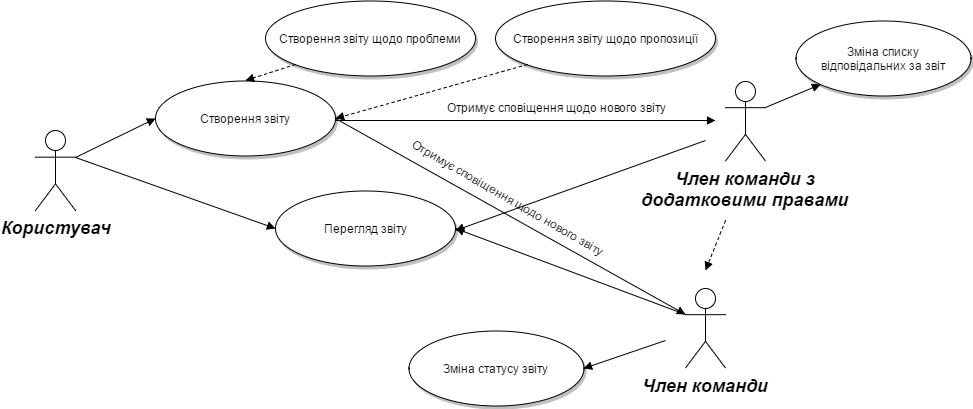
\includegraphics[width=1\textwidth]{diagram_usecase_1}
\caption{Механізм роботи зі звітами у вигляді діаграми прецедентів}
\end{figure}

\subsection{Формулювання та аналіз вимог за допомогою діаграми діяльності}

Процес створення звіту, що знаходится в процесі обробки персоналом проекту, має трьох основних учасників: користувач, відповідальний член команди, а також член команди з правом назначення відповідальних за звіт. Щоб звіт дійшов до стадії "в процесі"\mbox{}, після створення користувачем звіту його повинен перегланути член команди, що має право назначення відповідальних та назначити відповілальних за цей звіт осіб. Після цього, відповідильний член команди може назначити звіту той статус, який вважає потрібним, і, в тому випадку, якщо це доцільно, приступити до вирішення проблеми/впровадження нового функціоналу, при цього змінивши статус звіту на "в процесі".

% TODO Note that quote and coma does not appear in text!!! I'm not sure how easy or hard is to change quote's options, and what are best practice; commonly, I simply use either << and >> (ёлочки) or `` and '', AVOIDING " and ". It's surely one of common practices, but I'm not sure, is it the better. If there are some reasons to leaves quotes as is, change ", to "\mbox{}, If you use \enqoute{...} later, it may be a good idea to use it over all text

\begin{figure}[H]
\centering
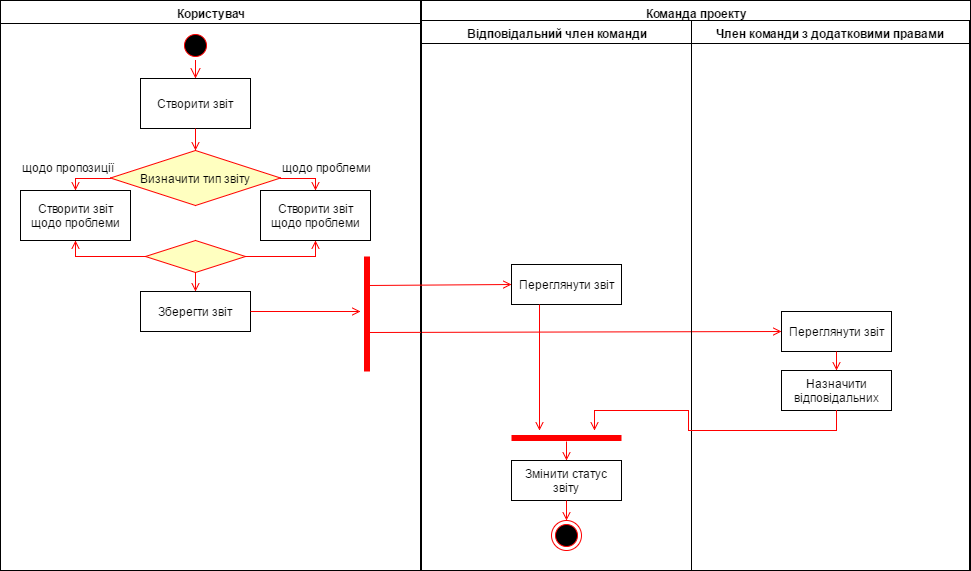
\includegraphics[width=1\textwidth]{diagram_activity_1}
\caption{Механізм роботи зі звітами у вигляді діаграми діяльності}
\end{figure}

\subsection{Аналіз вимог за допомогою діаграми послідовності}

При створенні звіту, користувач може побажати прикріпити важливу інформацію, пов'язану з цим звітом. В такому випадку, йому клієнтський додаток повинен спочатку завантажити додаткову інформацію на спеціально відведений для цього сервер, і вже потім, якщо користувач має на це право, оновити дані звіту, додавши до них посилання на додаткову інформацію, як зображено на діаграмі~\ref{figure_diag_seq_1}.

\begin{figure}[H]
	\centering
	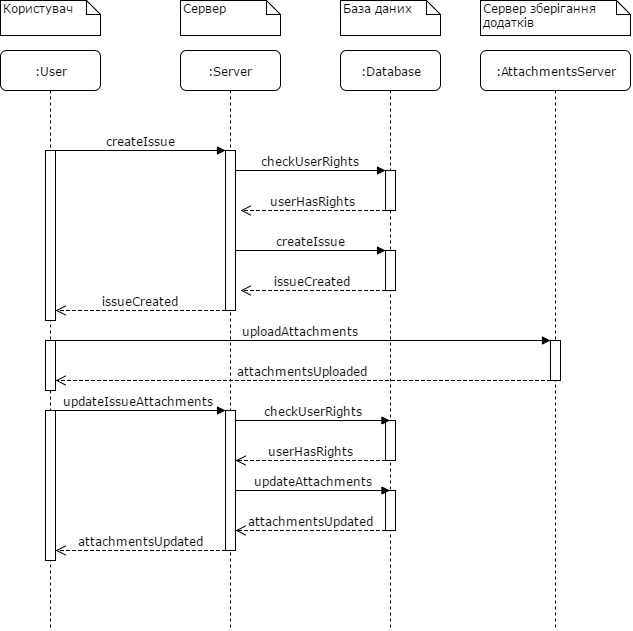
\includegraphics[width=1\textwidth]{diagram_seq_1}
	\caption{Механізм створення звіту з додатками у вигляді діаграми послідовності}
	\label{figure_diag_seq_1}
\end{figure}

\subsection{Аналіз вимог за допомогою діаграми комунікації}

Будь-яка система обліку повинна давати можливість пошуку та перегляду інформації. Багтрекінгові системи, як підвид систем обліку, в свою чергу також повинні надавати можливість створення звітів. Механізм перегляду проектів та звітів у вигляді діаграми комунікації зображено на діаграмі \ref{figure_diag_comm_1}.

\begin{figure}[H]
	\centering
	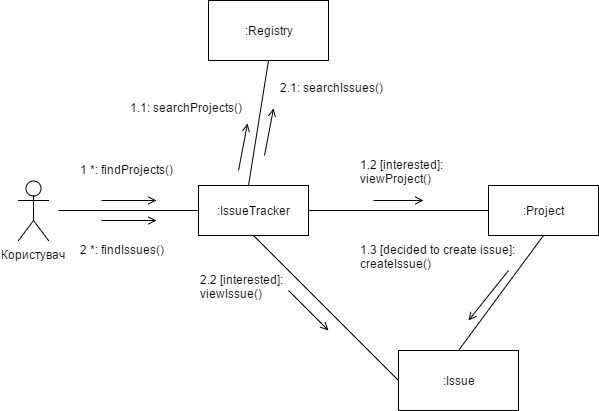
\includegraphics[width=1\textwidth]{diagram_communication_1}
	\caption{Механізм перегляду проектів та звітів у вигляді діаграми комунікації}
	\label{figure_diag_comm_1}
\end{figure}

% \section{Визначення поведінки об'єктів багтрекінгової системи}

\end{document}